\textsc{\large Reconocimiento del material de uso común en el laboratorio}\\

Describir los materiales de vidrio del laboratorio que se encuentran detallados en la Tabla 1. Especifique en cada caso si el material puede ser clasificado como: material volumétrico o no-volumétrico.

\begin{table}[ht!]
\caption{Materiales de uso común en el laboratorio.}
    \centering
    \begin{tabularx}{\linewidth}{|>{\hsize=0.2\hsize}C|>{\hsize=0.2\hsize}C|>{\hsize=0.6\hsize}L|}
    \hline
    \textbf{Nombre} & \textbf{Imágen} & \textbf{Descripción y carácterísticas}\\\hline
    Name of the material & 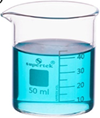
\includegraphics[trim=0 0 0 -5, scale=0.8]{images/p1.png} & Text that describes the characteristics of the material, this text is long to understand how this document works. Notice it is not necessary to use line breakers to keep writing. This can be done as long as you want.\\\hline
     & 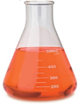
\includegraphics[trim=0 0 0 -5, scale=0.8]{images/p2.png} & \\\hline
     & 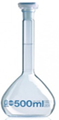
\includegraphics[trim=0 0 0 -5, scale=0.8]{images/p3.png} & \\\hline
     & 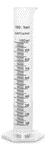
\includegraphics[trim=0 0 0 -5, scale=0.8]{images/p4.png} & \\\hline
     & 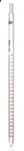
\includegraphics[trim=0 0 0 -5, scale=0.8]{images/p5.png} & \\\hline
     & 
\includegraphics[trim=0 0 0 -5, scale=0.8]{images/p6.png} & \\\hline
     & 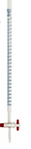
\includegraphics[trim=0 0 0 -5, scale=0.8]{images/p7.png} & \\\hline
    \end{tabularx}
\end{table}

Explique en que consiste la calibración de materiales volumétricos.\\[10pt]

Los materiales volumétricos muestran dentro de sus especificaciones las siglas: TC (o In) o TD (o Ex). Explique el significado de cada una.\\[10pt]

Los materiales volumétricos muestran dentro de sus especificaciones un valor de temperatura, típicamente 20 C, explique su significado.